% done 1

\section{Analyse du marché et des besoins, élaboration du cahier des charges}
In order to develop a product that could meet the needs of stuttering patients and speech therapists, I conducted research to define the exercises used by speech therapists during sessions with their patients. Since the project was to be completed in just 12 weeks, I decided to focus my research only online without contacting real speech therapists, which would have allowed me to more accurately identify real needs but would also have taken me a lot more time.

I also did a comparative study of the applications currently available on the Play Store, the summary table of this study is available in appendix \ref{appendix:market}. This study revealed a lack of complete application including different types of exercises. The applications currently available often focus on a single exercise. Also, no application proposes to make the link between stutters and their speech therapists.

In order to fully describe the purpose of the application, the context in which the application will be used (\textit{by whom? how? why? }), its functionalities and non-functional requirements (security, maintainability, \textit{scalability}, etc), I wrote a \textit{Software Requirements Specification (SRS)}. A \textit{SRS} is a document that gives a complete description of how the product is supposed to work, in particular this document describes the requirements for user interaction with the product and any constraints and non-functional requirements to be met (laws and regulations, protocol to be used, hardware limitations, security, etc.). The table of contents of this document is available in Appendix \ref{appendix:srs}. This document accurately describes the user interaction on the application summarized in the use case diagram in Figure \ref{fig:srs}. See Appendix \ref{appendix:srs_example} for an example of how to specify a use case.

\begin{figure}[h]
  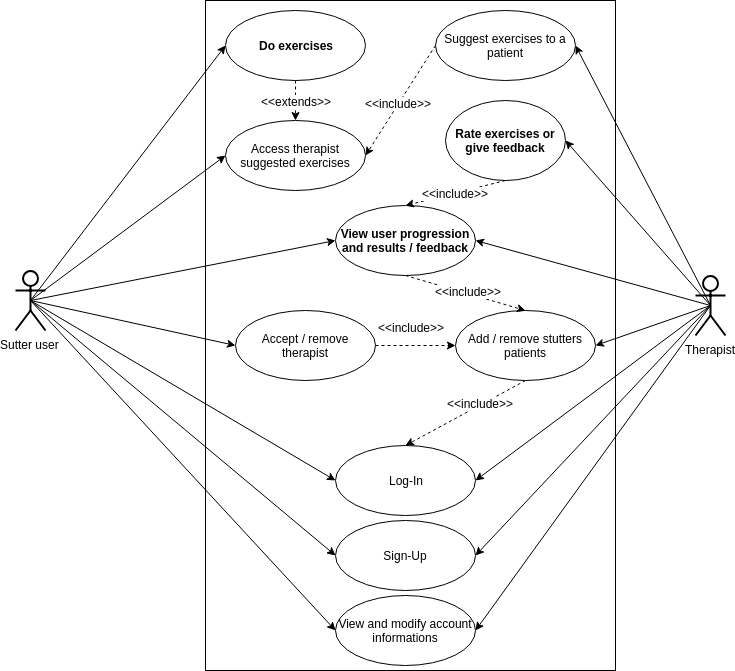
\includegraphics[width=.9\linewidth]{content/imgs/usecase.png}
  \caption{Use case diagram}
  \label{fig:srs}
\end{figure}

\subsection{Summary of the application specifications}
\label{sec:resume_cdc}

The application is intended for use by stuttering people and speech therapists. At the first start of the application the user will then have to choose whether to use the application as a stutterer or as a speech therapist.

\subsubsection{Stuttering users}

Stutterers will have a list of exercises to train to better control their speech flow. Each exercise will be customizable to suit the user's needs. In particular, the exercises may use resources that the user will have to read. These resources will have to be retrieved through a shared resource collection with several types of resources: words, sentences and texts. The stutterer will then be able to choose what type of resource he or she wants to train on. The exercises may also use other elements, such as a voice or video recorder to record the exercise. The user will be able to choose whether or not to activate these recorders. Here are 4 typical exercises that are part of the application:

\begin{itemize}
  \item \textbf{Metronome} : the stutterer trains to speak with a regulated rhythm using a metronome (a device that emits a signal -- visual and/or sound -- at regular time intervals);
  \item \textbf{Reading} : the stutterer speaks freely about resources of his or her choice (word, text, sentence);
  \item \textbf{Delayed Auditory Feedback (DAF)} : the stutterer speaks and then hears the return of his voice a few tens of milliseconds later;
  \item \textbf{Mirroring} : the stutterer trains to speak with a video feedback from his head to analyze his facial movements.
\end{itemize}

From the application specifications, I built the \textit{flowchart} (schematic representation of a sequence of actions) of user interaction on the different pages of the application, see appendix \ref{appendix:ihm}. The progression is based on the history of all the exercises performed. These exercises will include the possible voice or video recording, the resources used during the exercise as well as a feedback from the speech therapist (see below). The user's progress should also be graphically visualized using line charts illustrating the percentage of successful pronunciation of the words pronounced during the exercises.

The stuttering user may decide to synchronize his exercises in the cloud. To do this he will have to create an account with a name, an e-mail and a password. Once an exercise is synchronized in the cloud, it will be accessible by its speech therapist (if exists) who can then add a feedback on this exercise. Users who stutter can therefore add a speech therapist authorized to access all their synchronized exercises. To add a speech therapist they will need to know his or her personal identifier (see below). They will of course be able to revoke the access of this speech therapist to the exercises at any time.

\subsubsection{Speech therapists users}

To use the application's features, speech therapists will need to create an account (as for stuttering, with a username, e-mail and password). Once the account is created, the speech therapist will have access to his or her ID as well as a list of all the stuttering users who added him or her as their speech therapist. These users are called \textit{patients} for the speech therapist. The speech therapist will be able to visualize the progress of his patients. He may also remove patients from his list.















% eof
